\chapter{Style feature analysis}

\chapterquote{``Data! data! data!'' he cried impatiently. ``I can't make bricks without clay.''}{The adventure of the Copper Beeches\\Arthur Conan Doyle (1892)}

Of all the style metrics used, our goal is to determine which ones vary and differ depending on the recipient of the message. With this in mind, in this chapter we are going to analyse the resulting values of measuring each message with the previously explained system.

The first step in our analysis is to prepare the data. We have to categorise the different contacts depending on their relationship with the sender, choose the features that we are going to study and modify its values in order to have the data ready for being analysed. All of this is explained in Section \ref{sect:DatPrep}.

Once we have a defined the classification of each message, we are going to carry out a preliminary analysis of the style descriptors considered using clustering techniques (see Section \ref{sect:clust1}). This study will reveal us how our different categories will fit with the clusters given by these methods.

As we will see, due to the big amount of style metrics, to describe the features and the different categories of contacts will be too difficult. For this reason, a dimension reduction will be required. There is a wide variety of dimension reduction techniques, but we are going to start with the most popular of them: Principal Component Analysis (see Section \ref{sect:pca}). With this method, we will obtain results that does not take into account our categories. In addition to it, each category will not be well balanced. For these reasons, it will be necessary to use a less common dimension reduction technique: Gini Importance of Decision Trees (see Section \ref{sect:dectrees}). After the application of this machine learning method, the system is going to be reduced to only eight dimensions.

Finally, we will repeat the analysis with clustering techniques, but this time with the obtained eight dimensions (see Section \ref{sect:clust2}).

\section{Data preparation: e-mail classification, metrics choice and correlation analysis}\label{sect:DatPrep}
First of all it is necessary to classify the different recipients of the analysed messages. For this purpose, all the contacts (a total of 337 different e-mail addresses) have been divided into twelve categories depending on their relationship with the analysed user. These categories are: \textit{friend}, \textit{acquaintance}, \textit{company} (in this category are grouped all the company contacts with which the user has had a relationship to contract their service), \textit{university}, \textit{boss}, \textit{colleague}, \textit{professor}, \textit{relative}, \textit{stranger}, \textit{university position}, \textit{casting} (the people with which the user was in touch in order to manage a theatre casting belong to this relationship type) and \textit{company recruiting} (where are classified the e-mail addresses that the user contacted to be a candidate in a recruiting process).

Our style markers were applied to each message, so it is necessary to categorise the different e-mails. With this in mind, we determine the category of the message depending on its recipient(s). Classifying e-mails destined for a single e-mail account is a trivial problem (its category will be the one assigned to the message's recipient). We can also directly classify those messages whose recipients all belong to the same category. E-mails that have several receivers from different categories are automatically classified when they have only one addressee in the recipients field \textit{To} (they are grouped in that contact's category), which represents the main recipient(s) of the message, while the \textit{Cc} (Carbon Copy) and \textit{Bcc} (Blind Carbon Copy) fields have the purpose of keeping the addressees in there informed. Otherwise, we classify it one by one (there were only 14 messages out of 921 that we had to review) depending on the type of relationship we think indicates the wording of the message.

After this classification process, we obtained the distribution of relationship categories that we can see in Figure \ref{fig:distr}. As we can observe, we have not equally distributed classes and this represent a problem in our data analysis. Indeed, the biggest class (the \textit{professor} class) represents approximately $39.41$\% of the total, while the second one (\textit{university position}) in size is the $13.25$\%. And, of course, both categories are far from the smallest class (\textit{acquaintance}) which only represents approximately $0.33$\%. Despite this unbalanced distribution between the different categories, we will analyse this data set and obtain conclusions in order to detect the most significant features for differentiating the writing style based on the recipient of the e-mail. We have to take into account that the conclusions will be closely linked to the data obtained given the small sample size.

\begin{figure}
	\centering%
	\centerline{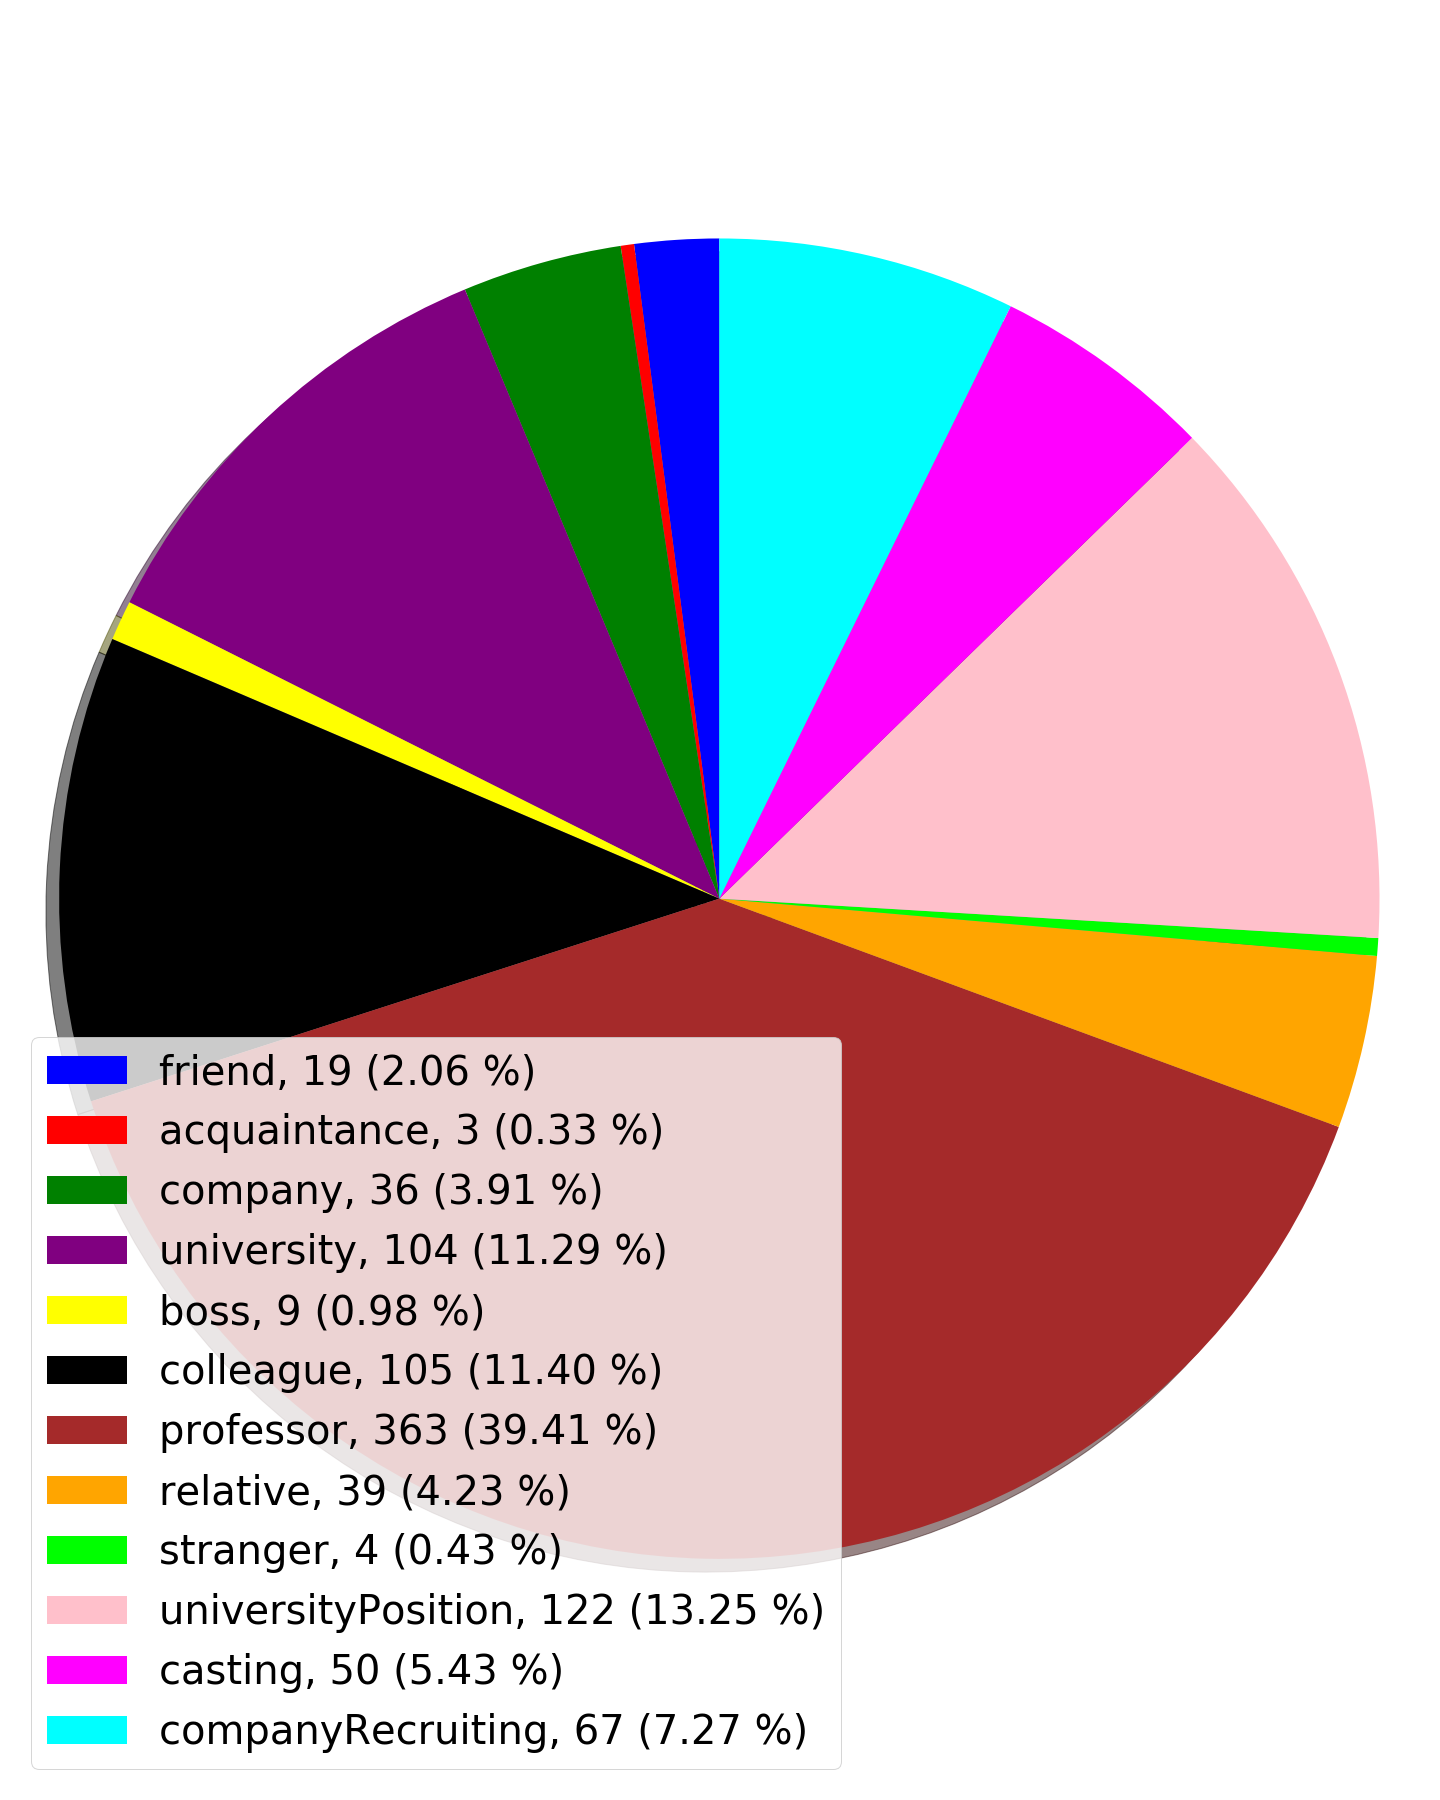
\includegraphics[width=0.5\textwidth]{Imagenes/Bitmap/classdistributionpie.png}}%
	\caption{Distribution of relationship categories}%
	\label{fig:distr}
\end{figure}

Once all e-mails are classified in our twelve categories, we have to choose which style features we are going to analyse. At first glance, there are features of each message (the attributes of the \textit{Metrics} class, which can be looked up in Section \ref{section:measmod}) from which we are not be able to extract significant numerical information, such as the sender of the e-mails (which is the same for all of them), the subject and the identifier of the thread they belong to (called \textit{threadId}). Besides, as the distribution of the different categories is too unbalanced, we risk losing underrepresented classes if a time-related weight is applied over the several metrics. For this reason, we decide not to take the date into account for our analysis.

\begin{figure}[p]
	\centering%
	\centerline{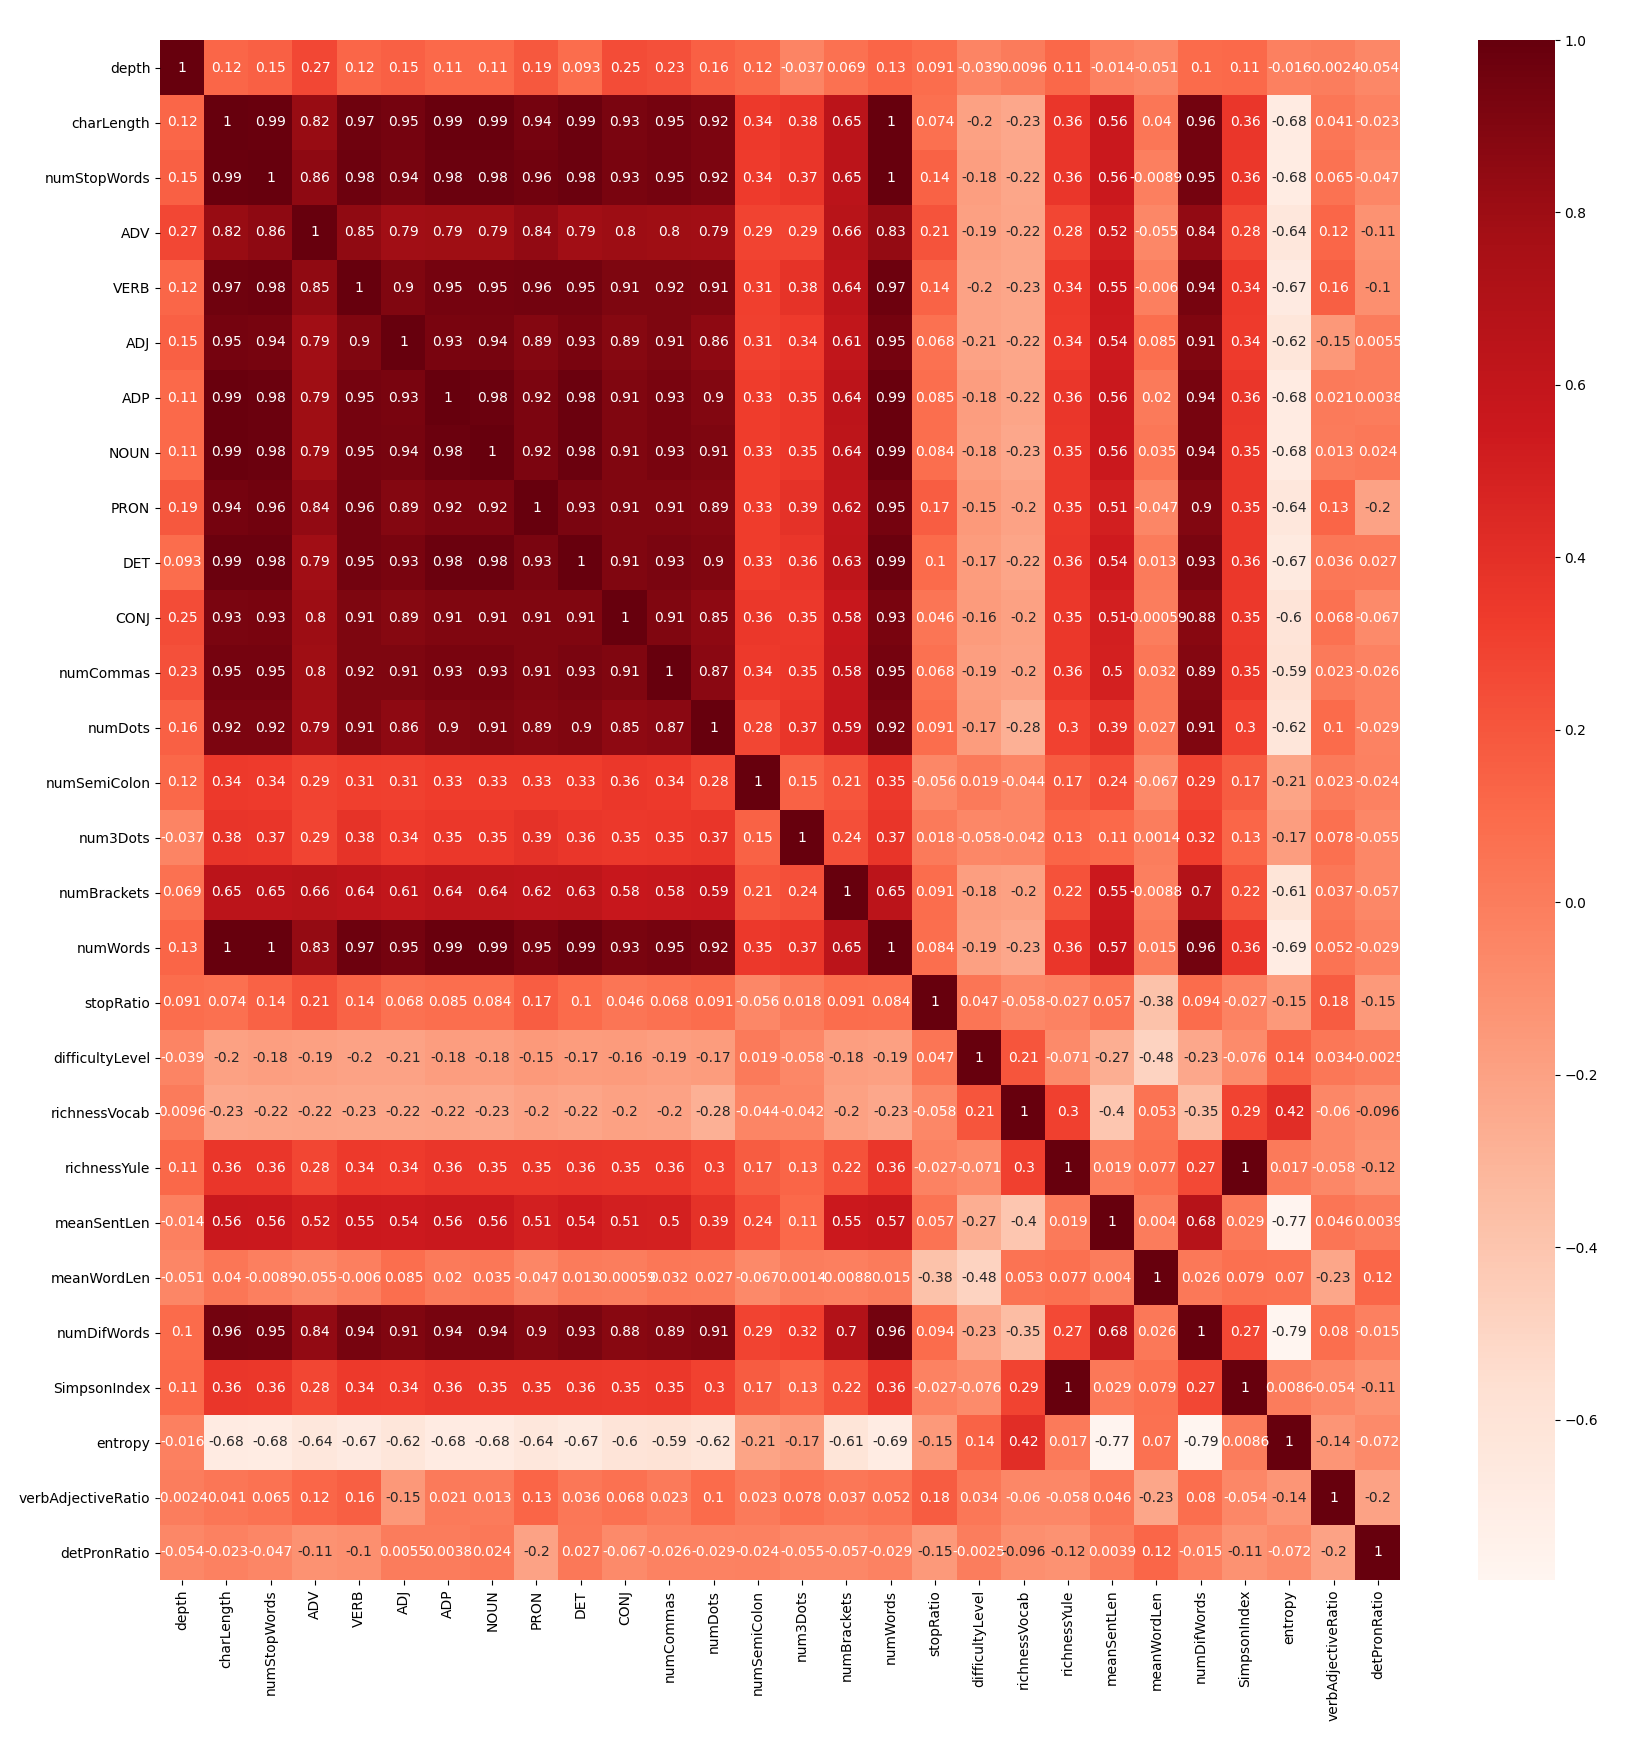
\includegraphics[width=0.98\paperwidth]{Imagenes/Bitmap/correlationmatrix.png}}%
	\caption{Pearson correlation coefficient between each pair of features}%
	\label{fig:correlation}
\end{figure}

In addition to the mentioned features, we have removed from our data set the following writing style markers: \textit{metricsSentences}, \textit{wordLength}, \textit{sentLength}, \textit{sentNumWords} and \textit{wordsAppearance}. All of them describe a distribution of a style feature (or several as the \textit{metricsSentence} attribute) through a dictionary or list structure, which are excessively complex to manipulate with the rest of the style features using common machine learning techniques. Furthermore, they would produce a big amount of NaN (Not a Number) values in our data set, because of the diversity in the number of sentences and words used in each e-mail (for instance if a message has an only sentence, all the style metrics related to the subsequent sentences will have a NaN value).

Therefore, we are going to work with 27 writing style markers, the depth of the message (perhaps we can find significant conclusions with this parameter) and the identifier of each message as index of each of the rows of our data set.

E-mail messages, by nature, do not contain a constant number of words from message to message. To overcome this variable and now that we have decided the style characteristics that we are going to study, the features are normalized, because techniques that require it (such as the K-Means algorithm) are used. Besides, we are going to find some NaN values, for example in \textit{verbAdjectiveRatio} and \textit{detPronRatio} in the messages where there are not adjectives or pronouns, respectively. The solution to overcome this problem, due to some algorithms do not admit data set with this type of values, is to assign the value of the arithmetic mean in the sample of individuals in the category to which the message belongs of the style marker in question, when it will be necessary. In other words, if an e-mail of the category $C$ has a NaN value in the style metric $M$, it will be replaced by the value of the arithmetic mean of the feature $M$ of the rest of the messages of class $C$.

It would be desirable to be able to visualize the main descriptive statistics to get an idea of each of the metrics. Nevertheless, given the big amount of style markers, the visualization becomes very complicated. For this reason, in the following sections, we try to reduce the dimensionality of the system in order to be able to explain the main characteristics and describe the writing style.

Before starting with the data analysis, we are going to study the relationship between each selected feature. To carry it out, the Pearson correlation coefficient \citep{benesty2009pearson} is going to be calculated between each pair of style markers. It is a measure of linear dependence between two quantitative random variables. Unlike covariance, Pearson's correlation is independent of the scale of measurement of the variables. Less formally, we can define Pearson's correlation coefficient as an index that can be used to measure the degree of relationship of two variables as long as both are quantitative and continuous. It has a value between $-1$ and $+1$, where 1 is total positive linear correlation, $0$ is no linear correlation, and $-1$ is total negative linear correlation.

As a result of the calculation of the Pearson correlation coefficient, we obtain the heat map of the Figure \ref{fig:correlation}. Logically, there is a positive linear correlation between those metrics that are strongly influenced by the length of the message. These pairs of style markers represent almost all results obtained close to the value 1. Moreover, there is a total positive linear correlation between Yule's Characteristic and Simpson's Index, which was predictable given the definition of one style feature with respect to the other (see Section \ref{ssect:vocabf}). These relationship will be taken into account during the analysis of the data.

\section{Preliminary analysis of the metrics considered using clustering techniques}\label{sect:clust1}
In an initial approach, we are interested in knowing how well metrics fit our twelve category classification. To achieve this, we have executed two popular clustering algorithms which are going to group our set of elements (composed of the different style features) in such a way that members of the same group (called a cluster) are more similar in one way or another. These algorithms are K-Means \citep{hartigan1975clustering} and DBSCAN \citep{ester1996density}.

\begin{algorithm}
	\begin{algorithmic}[1]
		\REQUIRE Data set $X$ (represented as a matrix whose columns are the features and whose rows are the different samples) with missing values, number of clusters $k$ and the maximum number of iterations to perform $maxiter$.
		\ENSURE A vector $labels$ that indicates to which cluster each element belongs and a data set $X^\prime$ which is a copy of $X$ with the missing values filled in.
		\STATE $X^\prime = X$
		\STATE $missing = $ list of positions (pair of rows and columns) of the missing values of $X$
		\FOR {$(row, column)$ in $missing$}
		\STATE $X^\prime[row, column] = mean(X[, column])$
		\ENDFOR
		\STATE $i = 1$
		\STATE $converge =$ \FALSE
		\STATE $prevlabels, prevcentroids = KMeans(init = random, k, X^\prime)$
		\FOR {$(row, column)$ in $missing$}
		\STATE $X^\prime[row, column] = prevcentroids[prevlabels[row]][column]$
		\ENDFOR
		\WHILE {$i < maxiter$ $\land$ $\lnot converge$}
		\STATE $labels, centroids = KMeans(init = prevlabels, k, X^\prime)$
		\FOR {$(row, column)$ in $missing$}
		\STATE $X^\prime[row, column] = centroids[labels[row]][column]$
		\ENDFOR
		\STATE $converge =$ $(prevlabels == labels)$
		\IF{$\lnot converge$}
		\STATE $prevlabels = labels$
		\STATE $prevcentroids = centroids$
		\STATE $i = i + 1$
		\ENDIF
		\ENDWHILE
		\RETURN $labels, X^\prime$
	\end{algorithmic}
	\caption{K-Means with missing values}\label{alg:kpod}
\end{algorithm}

Both algorithms require a parameter (in the case of K-Means the parameter is the number of clusters and in the case of DBSCAN the threshold distance that determines a neighbourhood of elements) which has to be defined before their execution. To make the decision of the initial value of the parameter there are methods based on the internal and cluster dispersion obtained. For this purpose, measures are taken to help the decision, such as the Silhouette Coefficient \citep{rousseeuw1987silhouettes}. It is a method of interpretation and validation of consistency within clusters of data. The technique provides a succinct graphical representation of how well each object has been classified. The best value is 1 and the worst value is -1. Values near 0 indicate overlapping clusters. Negative values generally indicate that a sample has been assigned to the wrong cluster, as a different cluster is more similar. Likewise, we can obtain a general idea of the behaviour of the clustering by calculating the mean Silhouette Coefficient for all samples.

Furthermore, we need to assess how much our classification resembles the clusters obtained after the execution of each of the algorithms. For this evaluation, we can use the Adjusted Rand Index, which is a form of the Rand index \citep{rand1971objective} that conforms to the random grouping of elements. The Adjusted Rand index is thus ensured to have a value close to 0.0 for random labelling independently of the number of clusters and samples and exactly 1.0 when the clusterings are identical (up to a permutation).

Due to the presence of NaN values, we are not able to use the K-Means algorithm directly on the data. Instead of replacing the NaN values as we have explained in Section \ref{sect:DatPrep}, we are going to use a slight variation from the K-POD algorithm \citep{chi2016k}, which runs K-Means iteratively while it modifies the cells where the value is missing by assigning the value of the centroids. The algorithm that we are going to use, similar to the K-POD, is the one shown in Algorithm \ref{alg:kpod}, where we have two invoked functions. The first one is \textit{mean}, which returns the mean of the given array without taking into account the missing values. The second one, \textit{KMeans}, is a function that applies the K-Means algorithm given a set of initial centroids (or it will generate them randomly), the number of clusters and the dataset. It returns an array as long as the number of rows of the given dataset which indicates the cluster index (through an integer) that each element belongs to and the coordinates (features values) of the centroid of each cluster (it will be a matrix with as many rows as the number of cluster and as many columns as the numbers of features).

Now that we have chosen the algorithm, we execute it with different $k$ parameter (the number of clusters). The rest of the input will be the normalised data with the NaN values and with a maximum of 100 iteration. With each $k$-dependent execution, we will calculate the Silhouette Score (which is the mean of the Silhouette Coefficient of all samples) and the Adjusted Rand Index given the real classification. As a result of this we obtain Figures \ref{fig:nkmeanssil} and \ref{fig:nkmeansari}.

\begin{figure}
	\hspace{-1cm}\begin{minipage}[b]{0.4\paperwidth}
	\centerline{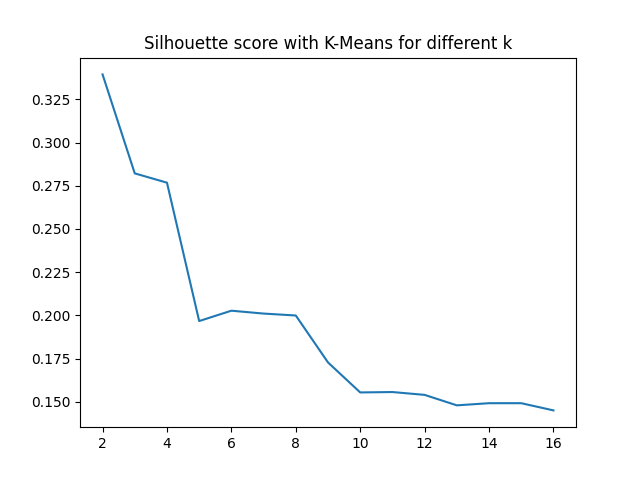
\includegraphics[width=\textwidth]{Imagenes/Bitmap/Clustering/normkmeanssil.png}}%
	\caption{Silhouette Score with K-Means for different $k$}%
	\label{fig:nkmeanssil}
	\end{minipage}
	\hspace{0.4cm}
	\begin{minipage}[b]{0.4\paperwidth}
		\centerline{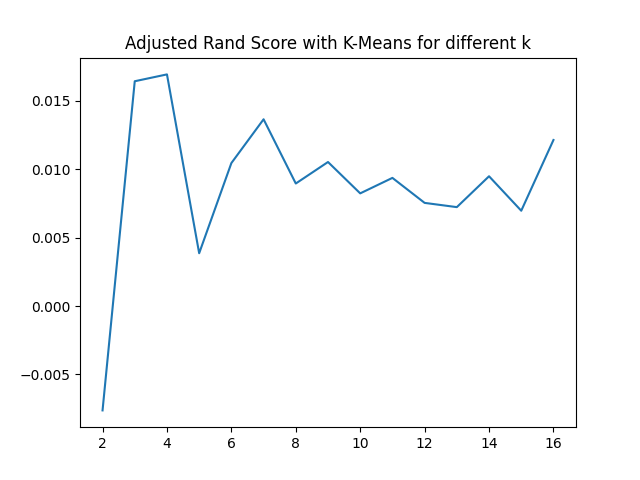
\includegraphics[width=\textwidth]{Imagenes/Bitmap/Clustering/normkmeansrand.png}}%
		\caption{Adjusted Rand Index with K-Means for different $k$}%
		\label{fig:nkmeansari}
	\end{minipage}
\end{figure}

In respect of the Silhouette Score analysis (which is shown in Figure \ref{fig:nkmeanssil}), with the given values, we are able to claim that, in general, as the number of groups increases the Silhouette Score decreases. This fact indicates us that the best number of clusters in order to achieve a good differentiation between each group of elements is two, which is not in line with our classification model. Not surprisingly, these results, which do not fit well in the established categories, are accompanied by poor values of the Adjusted Rand Index. As we can observe in Figure \ref{fig:nkmeansari}, all the obtained values with any number of cluster is very close to zero, which means, as we have previously explained, that the obtained classification does not match with ours.

In the case of DBSCAN algorithm, we are going to replace the missing values as we have explained in Section \ref{sect:DatPrep}. This clustering technique needs two different parameters: the threshold distance that determines a neighbourhood of elements (denoted by $\varepsilon$) and the minimum number of elements that forms a cluster. We will assign the value of three to this last parameter. This choice is motivated by the distribution between the different categories that we have previously defined. As we can observe in Figure \ref{fig:distr}, the smallest class has three elements in it, so it would not be consistent with our classification if a minimum number bigger than three is established. Moreover, the value of one does not make sense, since all the points of your data set will be a cluster (we would lose the possibility of detecting noise which is one of the advantages of DBSCAN over K-Means), and with 2 the result will be the same as the hierarchical cluster \citep{nielsen2016hierarchical} with the single-link metric, with the cut at the height of the dendrogram $\varepsilon$.

As we have done with K-Means, we are going to execute the DBSCAN algorithm with different $\varepsilon$ parameters. Besides, both the euclidean and manhattan metric are going to be used for this analysis. However, we will get similar results in both cases, so we are going to present the values obtained with the euclidean metric (see Figure \ref{fig:dbscaneu}).

\begin{figure}[t]
	\centering%
	\centerline{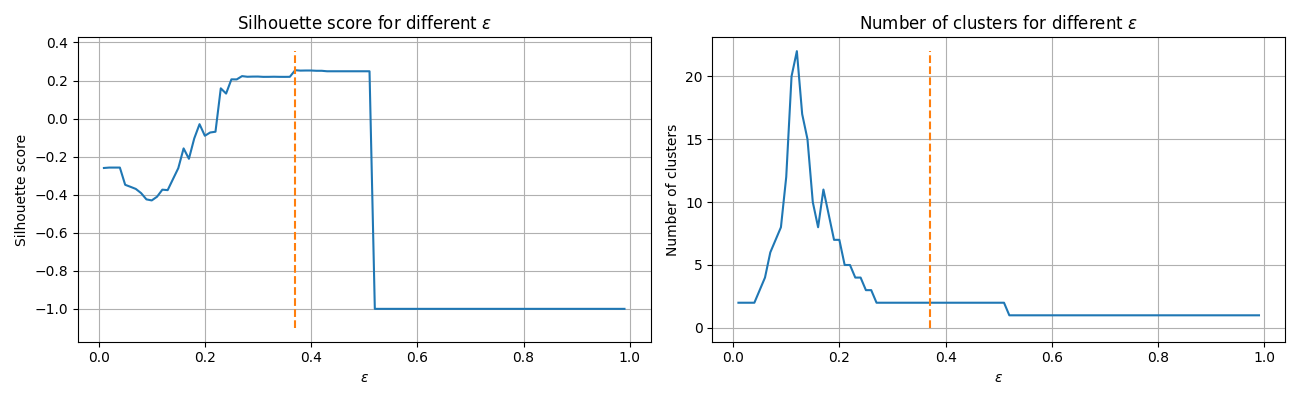
\includegraphics[width=\textwidth]{Imagenes/Bitmap/Clustering/dbscansil.png}}%
	\caption{Results of DBSCAN execution with euclidean metric}%
	\label{fig:dbscaneu}
\end{figure}

As in the case of the K-Means algorithm, we can find the maximum Silhouette Score with two clusters, which is not in line with our classification model. Furthermore, as we can see in Figure \ref{fig:dbscanari}, we find again values very close to zero in the Adjusted Rand Index analysis.

In conclusion, using the clustering techniques to classify the messages according to the selected metrics, as expected, we do not obtain significant results that fit our model or allow us to group the different e-mails in another way. One of the problems found to achieve this is the great amount of states that each element has, that is, the high number of dimensions of the system. We also find this inconvenience when we try to get the main statistics of the different features that describe the messages. Therefore, it is an issue that must be addressed (the reduction of dimensionality), especially trying that this reduction serves to adapt to the categorization carried out or to obtain a smaller number of parameters that define the writing style.

\begin{figure}[h]
	\centering%
	\centerline{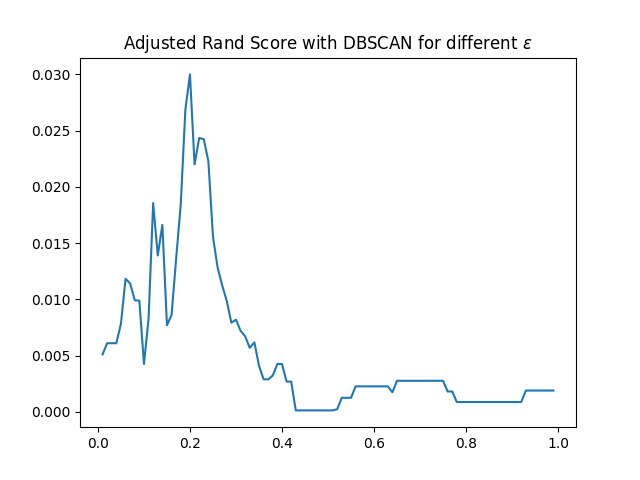
\includegraphics[width=0.5\textwidth]{Imagenes/Bitmap/Clustering/dbscanari.png}}%
	\caption{Adjusted Rand Index of DBSCAN with euclidean metric}%
	\label{fig:dbscanari}
\end{figure}

\section{Dimension reduction using Principal Component Analysis}\label{sect:pca}
In statistics, principal component analysis (PCA) is a technique used to describe a data set in terms of new, uncorrelated variables (components). Components are ordered by the amount of original variance they describe, so the technique is useful for reducing the dimensionality of a data set. Each of them is a linear combination of the set of features of the system. Therefore, if we know the weight assigned to each characteristic of the system, we are able to deduce the ``importance'' of each feature weighted by an specific explained variance.

For the PCA, the normalized data will not be enough. Of course, it will be necessary to replace the missing values as we explained in Section \ref{sect:DatPrep}, but also we are going to require a set of data with its features centred in zero, that is to say, that their mean must be zero. This transformation is called standardisation and we will apply it to our dataset.

If the PCA is executed with as many components as features, the sum of the explained cumulative variance ratio of all components is always 1. In other words, if all the main components of a dataset are calculated, then, although transformed, all the information present in the original data is being stored. With this method, we are able to know the various components that we can obtain and their explained variance. Likewise, the behaviour of the cumulative variance ratio is defined by the curve shown in Figure \ref{fig:cumexpvar}.

\begin{figure}[h]
	\centering%
	\centerline{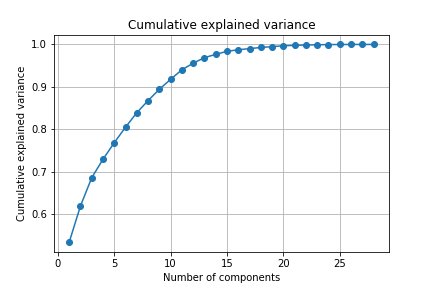
\includegraphics[width=0.7\textwidth]{Imagenes/Bitmap/PCA/cumexpvar.png}}%
	\caption{Evolution of cumulative explained variance ratio}%
	\label{fig:cumexpvar}
\end{figure}

Looking at Figure \ref{fig:cumexpvar}, we can affirm that around the 10 components, the increase of the explained accumulated variance stops being substantial and we reach a reasonable value of it. Hence, with the observed curve we are able to determine the suitable number of components. However, before delving into each of the components, let's study in more detail the distribution of the variance explained. For this purpose, we are going to represent the distribution of explained variance in a pie chart with which it will be easier for us to compare the different values of it. This graph is shown in Figure \ref{fig:expvarpie}.

\begin{figure}
	\centering%
	\centerline{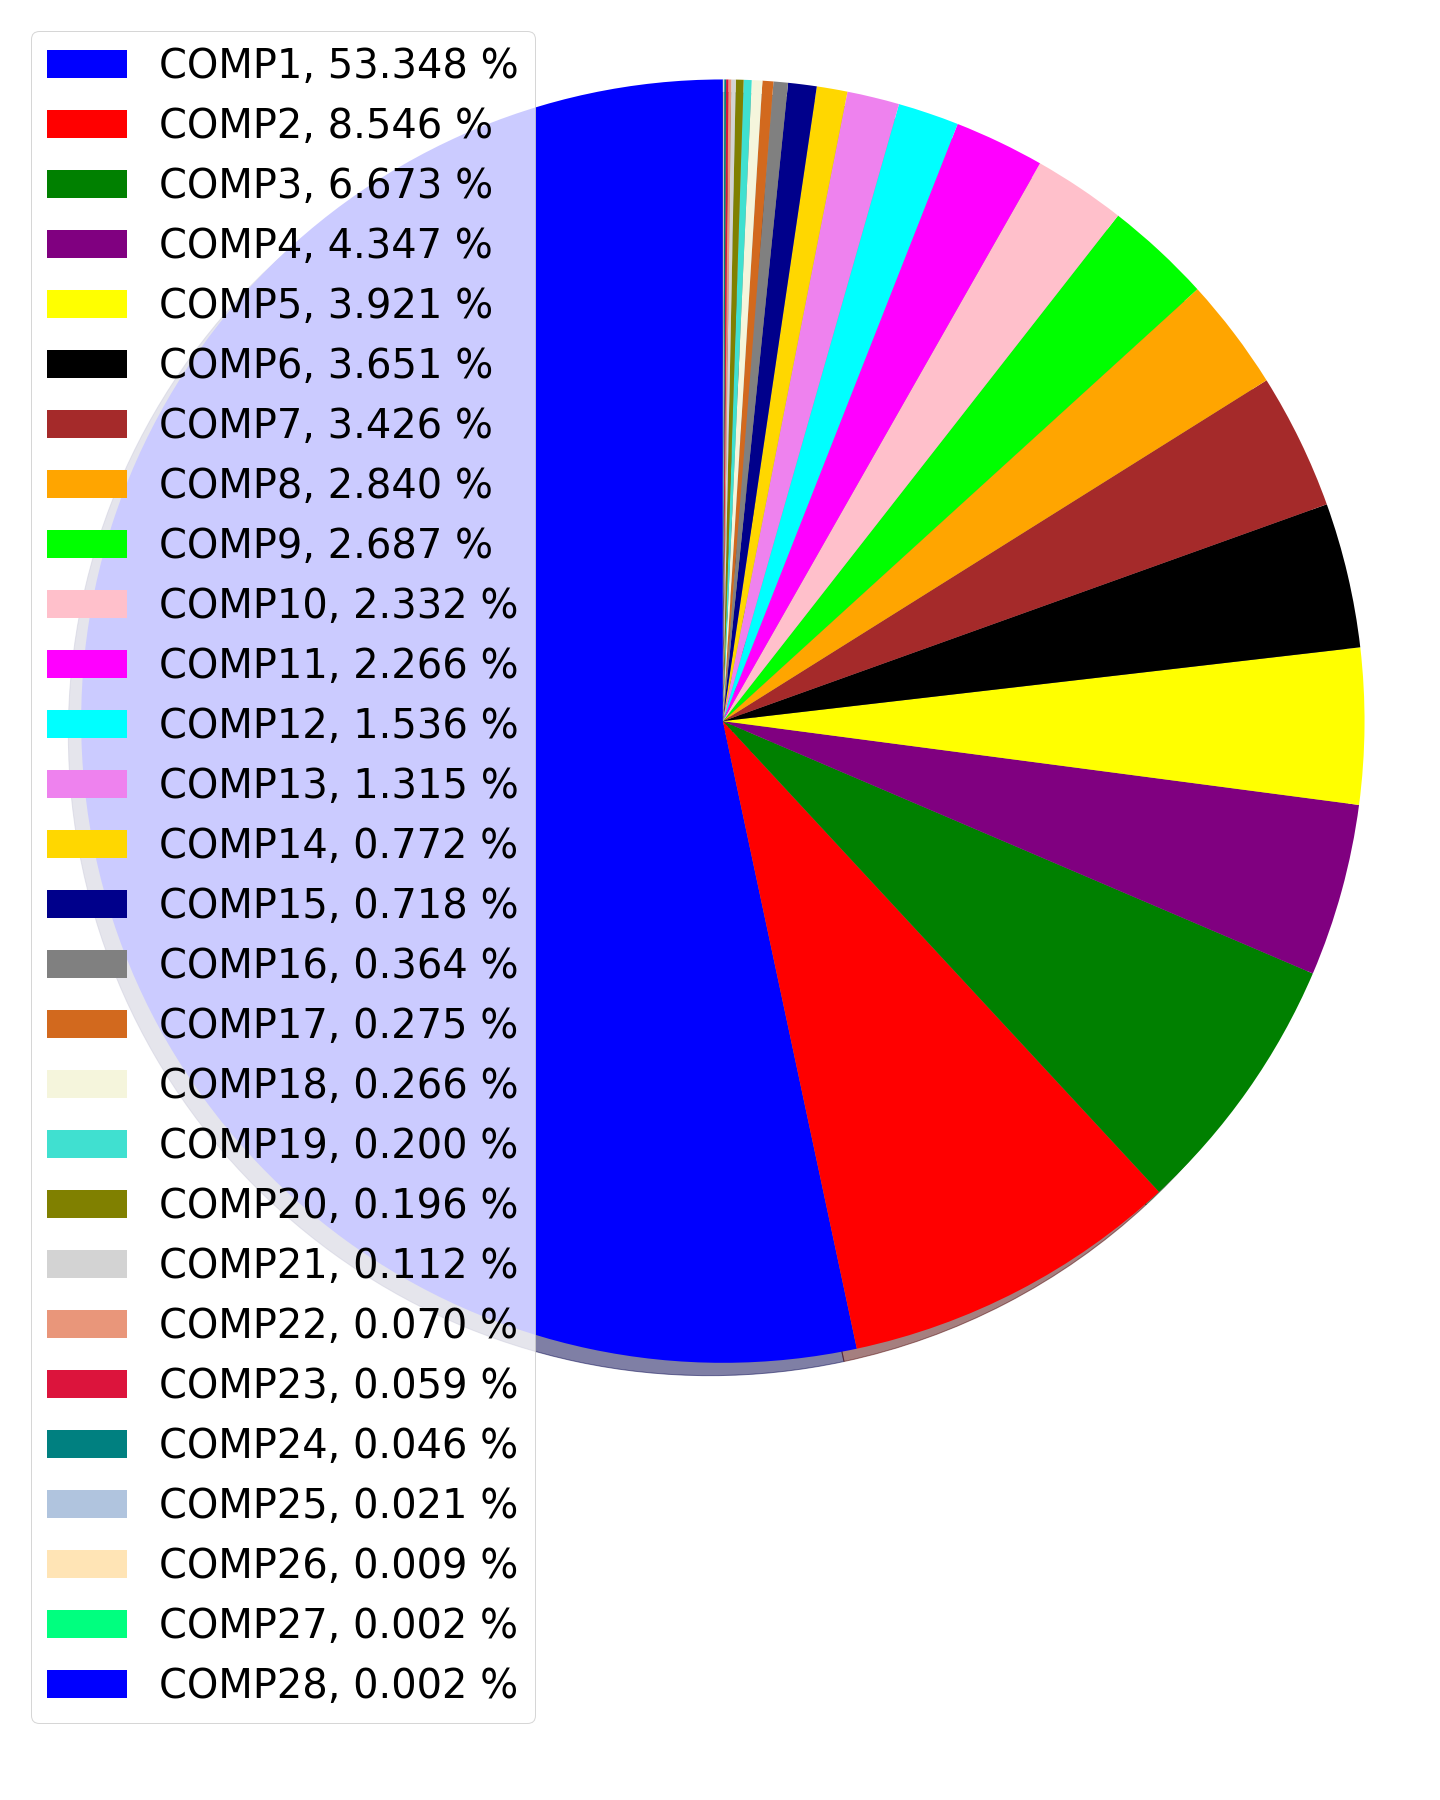
\includegraphics[width=0.5\textwidth]{Imagenes/Bitmap/PCA/expvarpie.png}}%
	\caption{Distribution of explained variance ratio}%
	\label{fig:expvarpie}
\end{figure}

Taking advantage of the information provided by the last graphic (Figure \ref{fig:expvarpie}) we can observe that the only component that has an explained variance ratio bigger than $10$\% is the first one. Besides, from the fourth one all of them has a value smaller than 5\% and from the thirteenth one the components have a poorly significant value. Nevertheless, we have to take into account that, given the distribution of our classification (see Figure \ref{fig:distr}), the losing of a small percentage of explained variance may mean missing information related to categories with few elements. This results from the fact that the PCA does not consider the appropriate classification during its execution.

In spite of the explained results in terms of components distribution, we could expect to obtain more clarifying values in the weights that define the components with higher explained variance ratio. Therefore, we will now know the linear combination of the first component with respect to the characteristics explained.

The best way to visualise the different linear combination weights is through a pie chart. This is because, with this graph, it is easy to compare the importance given to each dimension. In our Figure \ref{fig:comp0pie}, we have striped each linear combination which has a a negative weight and represented the absolute values of all coefficient. Since we are not so interested in the sense of each dimension in the definition of the first component, we will calculate the direction ratio that is assigned to each characteristic, for example if our system had two features (which is the same as saying that the system has two dimensions) and the direction ratio was greater in the first one, which we can represent on the abscissa axis, we would obtain a vectorial component whose representation in the common Cartesian plane will be ``more horizontal than vertical'', since the weight assigned to that dimension is greater. To find this direction ratio, we will divide the absolute value of the coefficient by the sum of the absolute value of each of the weights, that is to say, if a component is defined as follows:

$$
c_{i, k} = \sum_{j = 0}^N\lambda_{i, j}x_{k, j}
$$

Where $c_{i, k}$ is the value of the i-th component of the k-th e-mail, $N$ is the number of dimensions (28 in our case), $\lambda_{i, j}\in\mathds{R}$ is the linear combination coefficient (also called weight) of the i-th component for the j-th dimension and $x_{k, j}$ represents the j-th feature of the k-th message. Then, the direction ratio of the j-th characteristic of the i-th component is as follows:

$$
d_j = \frac{\lvert\lambda_{i,j}\rvert}{\sum_{j = 0}^N\lvert\lambda_{i, j}\rvert}
$$

The result of this operation will be the percentages that we can find next to each characteristic in the Figure \ref{fig:comp0pie}.

\begin{figure}
	\centering%
	\centerline{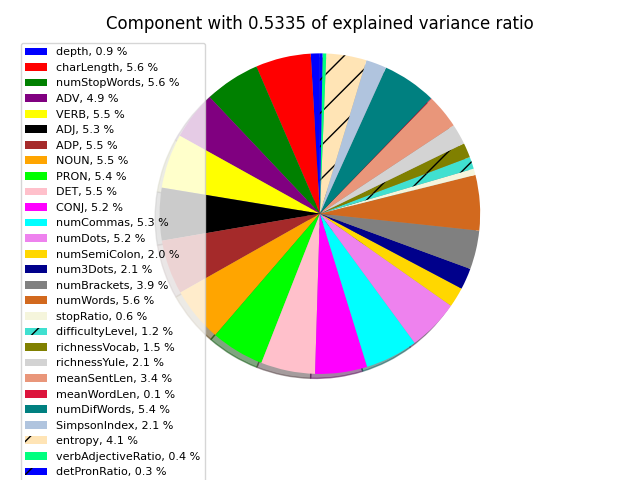
\includegraphics[width=0.9\textwidth]{Imagenes/Bitmap/PCA/comp0pie.png}}%
	\caption{Linear combination that defines the first component}%
	\label{fig:comp0pie}
\end{figure}

In addition to the problems of the choice about the number of components given our distribution in categories, we have a balanced assignment of weights of almost all the features in the first component, which has the highest explained variance with a ratio of 53.35\%. These information does not allow us to determine which style markers differentiate the categories of the messages. Furthermore, by not taking into account our classification, we can only state that the assignment of coefficients of the linear combination that defines the first component distinguishes the elements of the set equally, regardless of the class to which they belong.

As the rest of the components have an explained variance ratio smaller that 0.1, their direction ratios will not be sufficiently representative to overcome such a balanced distribution. For this reason, we can conclude that it is necessary to look for other method of dimension reduction which provides us information taking into account our classification and allows us to know which style metrics describe the different categories in the best possible way.

\section{Dimension reduction using Decision Trees}\label{sect:dectrees}
One method of machine learning, although not mainly used for dimensional reduction (there are some researchers that have studied the feature selection using them as \cite{sugumaran2007feature} and \cite{cho2011decision}), that takes into account a given classification is Decision Trees. A Decision Tree \citep{rokach2008data} is a prediction model, which given a set of data, makes logical construction diagrams, very similar to rule-based prediction systems, which serve to represent and categorize a series of conditions that occur successively, for the resolution of a problem. There are many algorithms to implement them, we are going to use an optimised version of the CART algorithm \citep{breiman1984classification} with entropy as its criterion.

The advantages of Decision Trees are that they take into account the defined categorisation, as it is a supervised machine learning classification method, and that they are very explainable. However, our purpose is to know the features that best describe the writing style based on the recipient, instead of classifying new messages. For this reason, we are going to make use of the structure of the constructed Decision Tree in order to measure the importance that each style metric has in it.

\begin{figure}
	\centering%
	\centerline{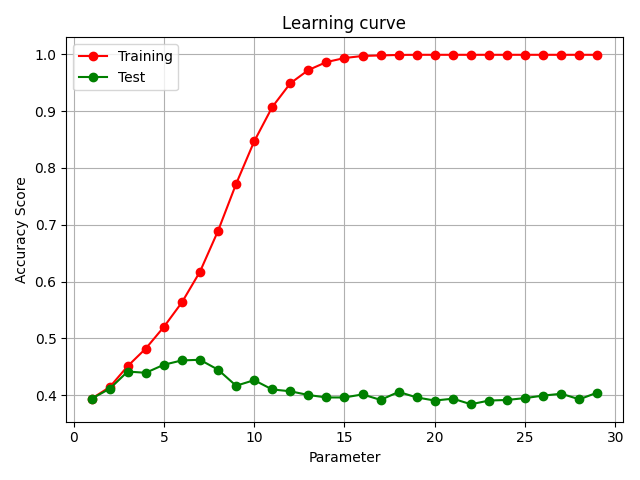
\includegraphics[width=0.7\textwidth]{Imagenes/Bitmap/DecisionTrees/learning28curve.png}}%
	\caption{Learning curve with the 28 chosen features}%
	\label{fig:learn28curve}
\end{figure}

A good intuition is to think that, in order to study the importance of a node, it is important to bear its depth in the tree in mind, because as lower is as more elements it differentiate. However, it will not be so useful if it just separate elements of the same class. Likewise, the number of samples that reach the node and its category is an important factor to keep in mind. Nevertheless, it will not be helpful if it maintains the proportion of each category in its child nodes. We are able to think many parameters that can have relevance in the definition of the importance of a node in the Decision Tree. In this case we are going to use the Gini Importance \citep{breiman2001random}, which is defined by the following expression:

$$
ni_j = w_jH_j - w_{left(j)}H_{left(j)} - w_{right(j)}H_{right(j)}
$$

Where $ni_j$ is the importance of node j, $w_j$ is the weighted number of samples reaching node j, $H_j$ is the entropy of node j, $left(j)$ is the child node from left split on node j and $right(j)$ is the child node from right split on node j. Consequently, the importance of each feature is defined by the following formula:

$$
fi_i = \frac{\sum_{j\in Nod(i)}ni_j}{\sum_{j\in Nod}ni_j}
$$

Where $fi_i$ is the importance of feature i, $Nod(i)$ is the set of nodes which split on feature i and $Nod$ is the set of all nodes. In our study we are going to use the normalised feature importance, which is defined by the following expression:

$$
nfi_i=\frac{fi_i}{\sum_{j\in F}fi_j}
$$

Where $nfi_i$ is the normalised feature importance and $F$ is the set of features. Once we have the expression required for the analysis of the importance of each feature, we are able to calculate the distribution of the importance of each style metric with our 28 chosen style markers. To build the Decision Tree, we have to decide the depth of it. To take this decision, we calculate the learning curve both in training set and test set, and obtain the curves that we can observe in Figure \ref{fig:learn28curve} (the normalised data was used for the calculation of learning curve, as well as in the construction of the Decision Tree). Thus, we will choose a depth that avoids the overlearning (which could be produced in values of depth with which the training accuracy score is 1) and the missing of information (depth with which the training accuracy score is less than 0.9). Our choice will be the depth whose training accuracy score is the interval $(0.9, 1)$ and its test accuracy score is maximum (in this case it is eleven, but later, when we had less features, it will follow this criteria).

Making use of the explained expressions for the calculation of the normalised feature importance, we can go through the created tree with the chosen depth in order to obtain the distribution of this value. The result is shown in Figure \ref{fig:nfi28}.

\begin{figure}
	\centering%
	\centerline{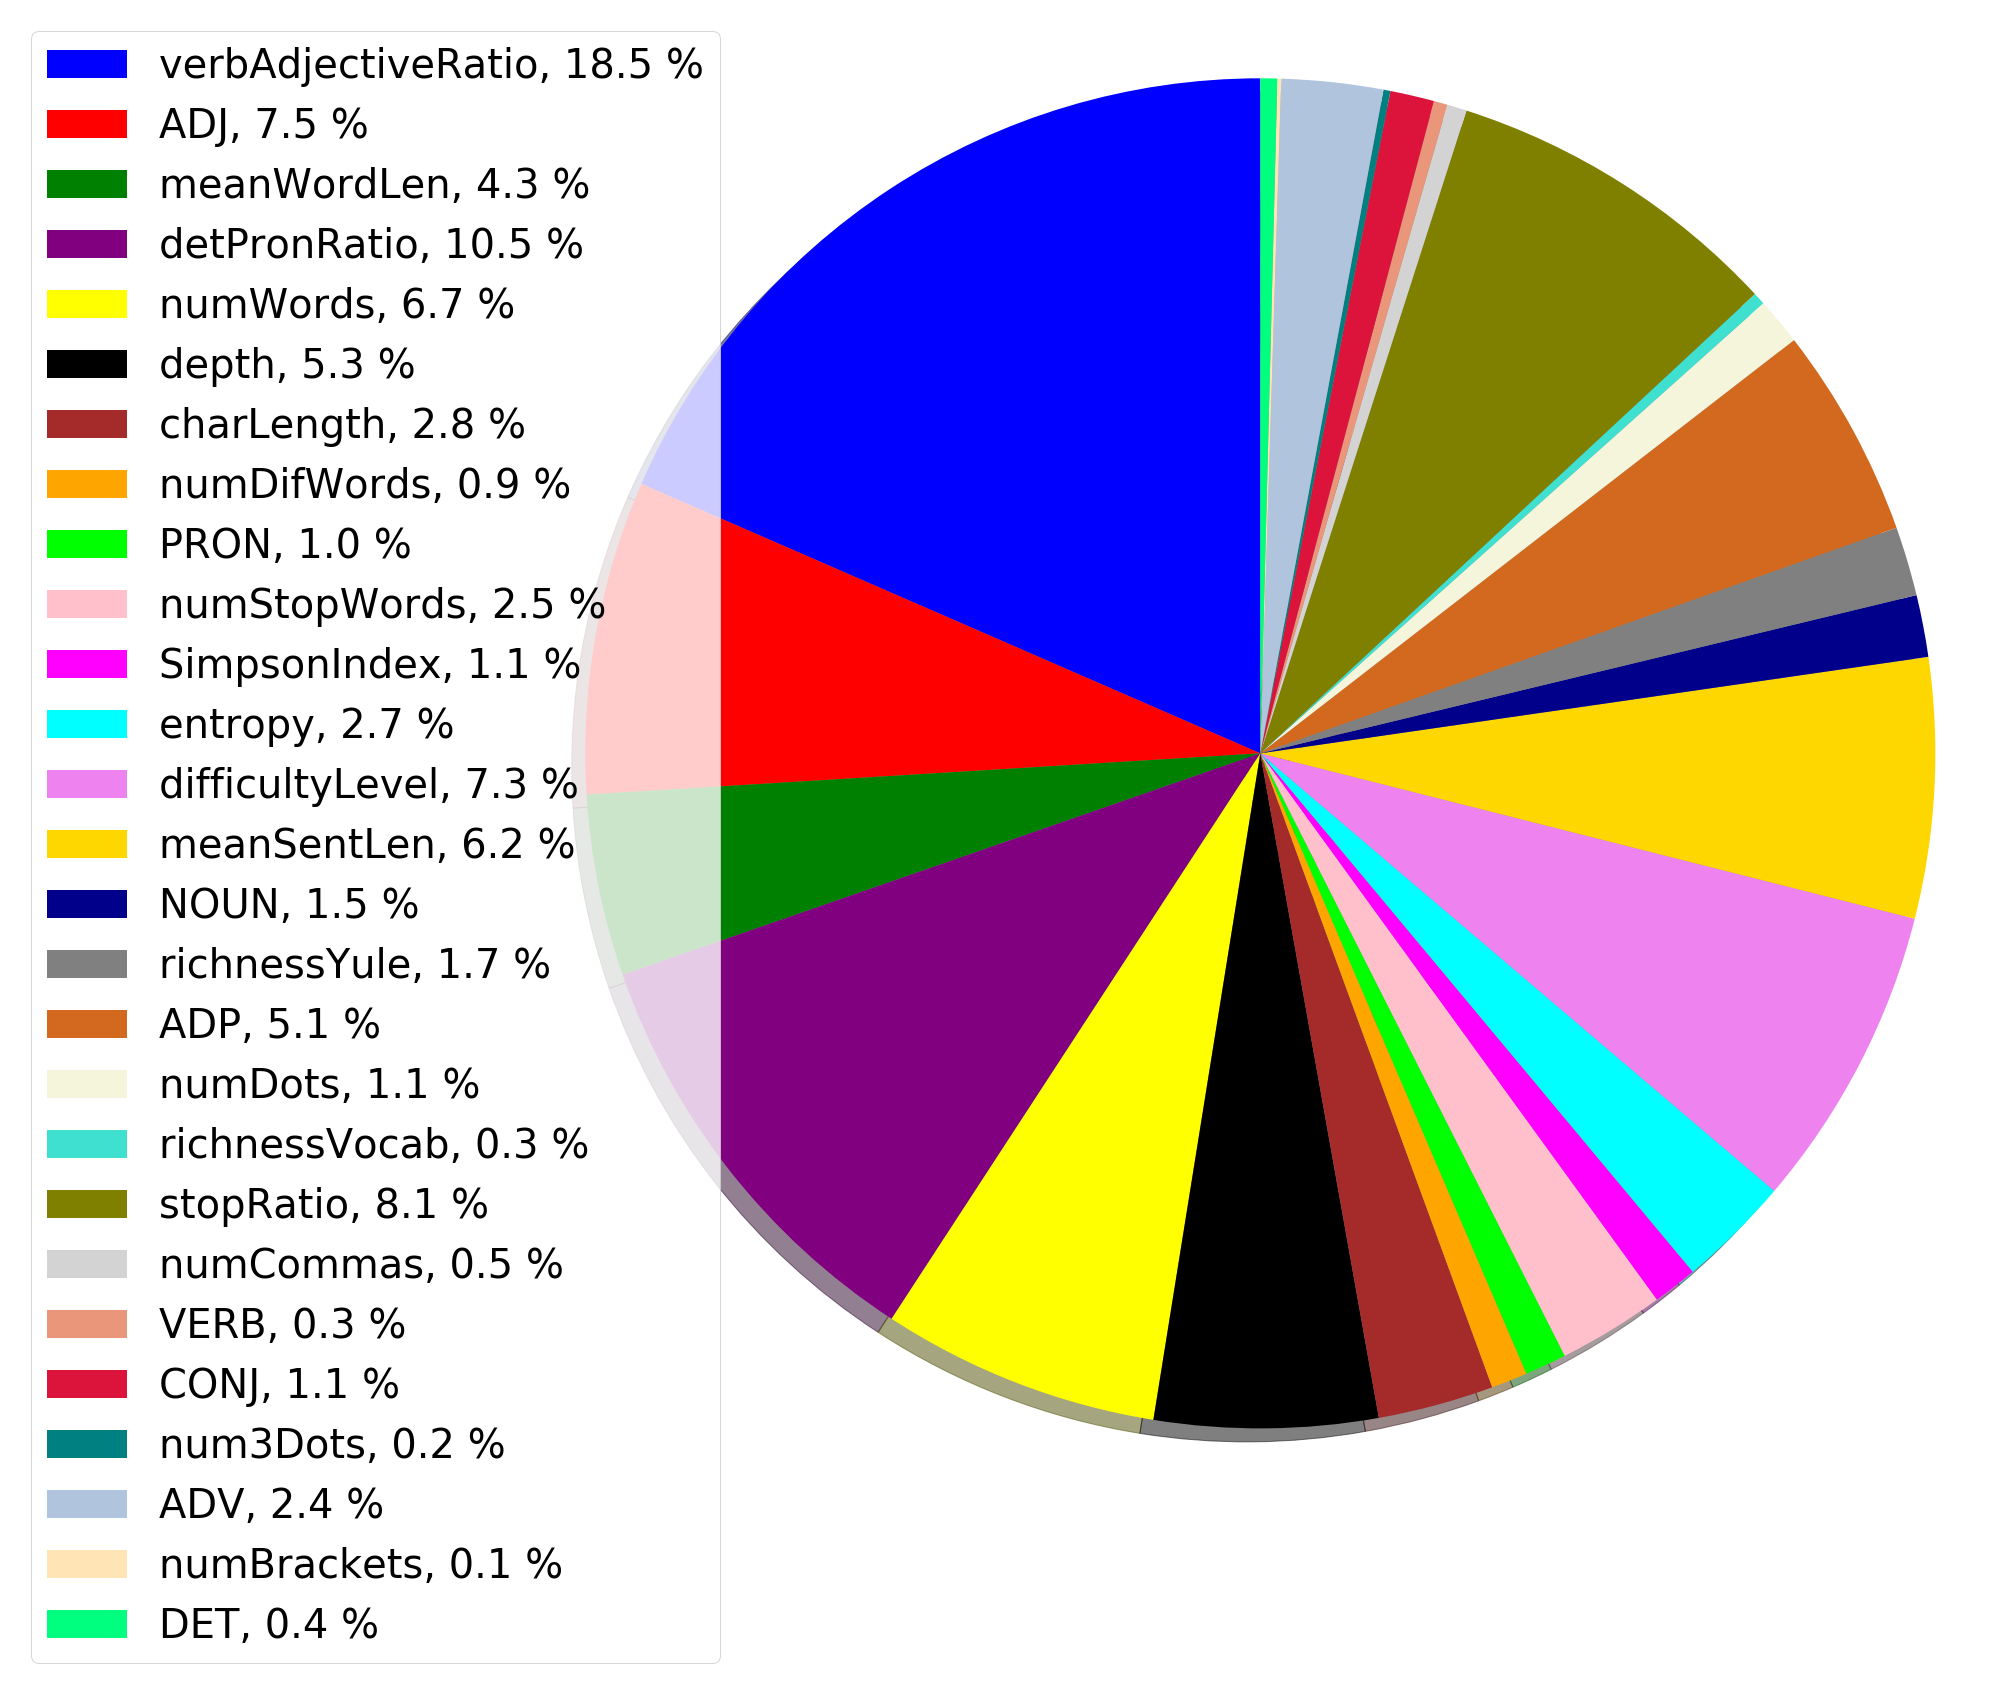
\includegraphics[width=0.8\textwidth]{Imagenes/Bitmap/DecisionTrees/pie28.png}}%
	\caption{Distribution of normalised feature importance with 28 features}%
	\label{fig:nfi28}
\end{figure}

As we can observe, the \textit{numSemiColon} characteristic has no importance in our constructed tree. Besides, \textit{verbAdjectiveRatio}, \textit{detPronRatio} and \textit{stopRatio} have the highest importance ratio and their related metrics (\textit{ADJ} and \textit{VERB}, \textit{DET} and \textit{PRON}, and \textit{numStopWords}, respectively) have a very small value. For this reason, we are able to claim that we can dispense with the related style features and \textit{numSemiColon} in order to describe the writing style. Therefore, we can construct another Decision Tree (by automatically taking a depth, as we have explained before) to calculate the importance ratio of each of the non-removed style markers. When we have the distribution of Gini Importance, we can removed again the non-important style metrics and those that have an extremely low importance ratio. By repeating this process, we are able to choose a small number of features which have a big importance ratio in the classification of the messages based on their recipients.

The learning curves of these iteration are all very similar to the one shown in Figure \ref{fig:learn28curve}. However, the evolution of the importance ratio of the style metrics is not uniform during all this iterative process. This behaviour could be seen in Figure \ref{fig:impcurv}.

\begin{figure}
	\centering%
	\centerline{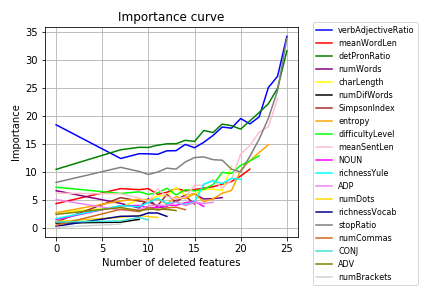
\includegraphics[width=0.9\textwidth]{Imagenes/Bitmap/DecisionTrees/limportancecurve.png}}%
	\caption{Evolution of importance ratio}%
	\label{fig:impcurv}
\end{figure}

Figure \ref{fig:impcurv} represents the importance ratio of each feature until it was removed from the set of style markers. The features that does not appear in the legend are those that were non-important in the first or second iteration, or were removed (such as the previously mentioned \textit{ADJ} and \textit{VERB}) before the second step.

Before detailing the different importance curves of each feature, there are some interesting general observations. Until the elimination of twenty features, which means having eight style metrics, it is always decided to dispense with some style marker whose importance is around 5\% compared to others that are above 10\%. From this point on, we see that characteristics with a more relevant importance start to be lost. From this fact we can deduce that keeping eight style metrics is a good principle to describe the style based on the recipient.

In general, the behaviour of the most of the features is constant. As we can observe, most of the last eight style markers were the most important features at the beginning of the process. Of course, little by little, some of the metrics experience an increase due to, as the sum of all the non-removed metrics importance is always the same, the ratio has to be distributed between a lower number of characteristics. However, this increase becomes remarkable as early as a big amount of style markers has been deleted (approximately from 20 removed features).

Thanks to the constant evolution of the importance of each metric, we can claim that most of the selected features (those which had not been removed until the number twenty), were those which had the highest values at the beginning; as well as, almost all of the deleted style markers when they have insignificant values of the ratio, were unimportant at the beginning. This fact allows us to assert that, given our dataset, our classification and our selected features, to add unimportant style markers does not excessively contribute to hide the really significant style descriptors.

Another possible assessment of the evolution of importance described by the Figure \ref{fig:impcurv} is that most of the features that are eliminated below 5\% of importance, before being so experience a slight decrease.

Going into more detail, the last eight selected features are: \textit{verbAdjectiveRatio}, \textit{detPronRatio}, \textit{meanSentLen}, \textit{meanWordLen}, \textit{richnessYule}, \textit{difficultyLevel}, \textit{stopRatio} and \textit{entropy}. All of them has an importance bigger than 8\% as we can see in the importance distribution of the Figure \ref{fig:nfi8}. Moreover, as we can check with Figure \ref{fig:correlation}, none of these metrics are directly correlated with each other.

\begin{figure}
	\centering%
	\centerline{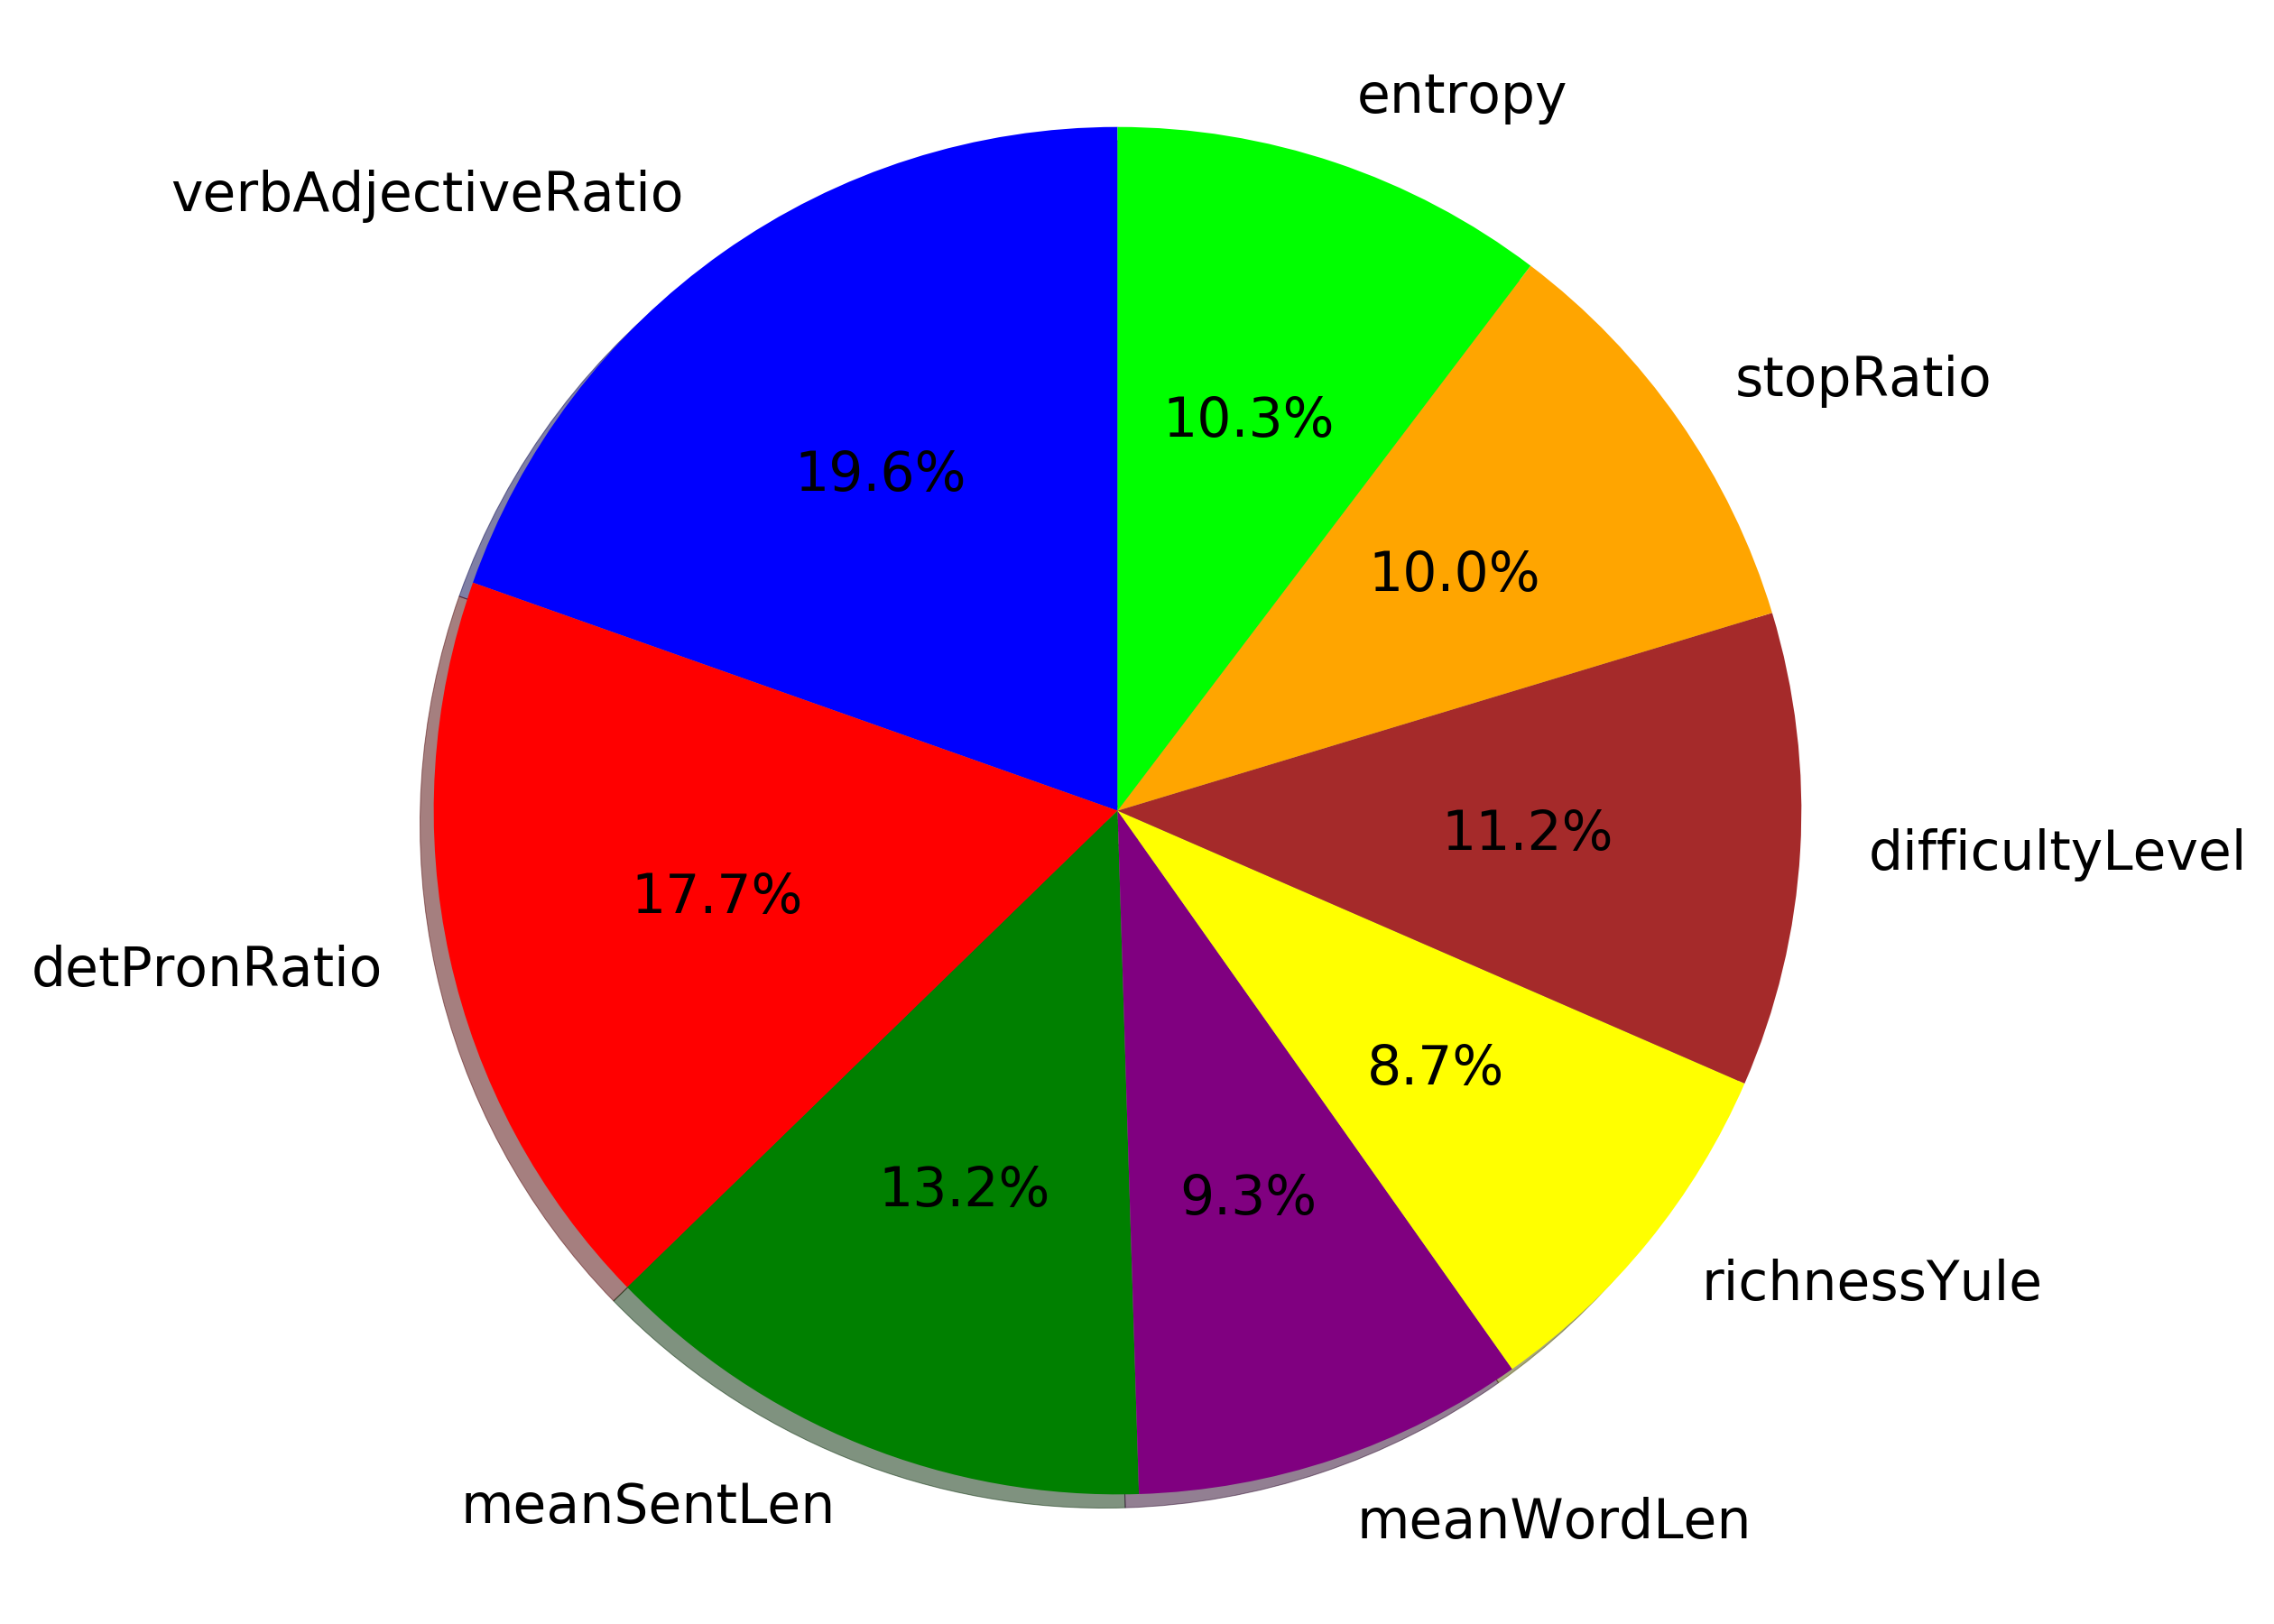
\includegraphics[width=0.8\textwidth]{Imagenes/Bitmap/DecisionTrees/pie8.png}}%
	\caption{Distribution of normalised feature importance with 8 features}%
	\label{fig:nfi8}
\end{figure}

In respect of the removed descriptors, some of them were deleted because they are related with another metric with has a bigger normalised feature importance. This is the case of \textit{ADJ}, \textit{VERB} (both related with \textit{verbAdjectiveRatio}), \textit{DET}, \textit{PRON} (this last two are related with \textit{detPronRatio}), \textit{numStopWords} (related with \textit{stopRatio}) and \textit{SimpsonIndex} (which is directly correlated with \textit{richnessYule}, due to their definitions). The unimportant style markers were also removed. In this case we have only two examples: \textit{numSemiColon} and \textit{num3Dots}.

On the other hand, we have deleted some style metrics due to their very low importance ratio and the existence of another style marker with a bigger value which is correlated with them. \textit{ADV}, \textit{ADP}, \textit{NOUN}, \textit{CONJ}, \textit{numCommas}, \textit{numDots}, \textit{numWords} and \textit{numDifWords} belong to this circumstances. The \textit{numBrackets} feature was removed only because of its extremely poor normalised feature importance (when it was deleted it had a value of 0.7\%).

We still have to explain the reasons why three style descriptors were eliminated. The \textit{depth} feature was removed because our purpose in this work is to develop a model which is based on the recipient of the message and not on its depth. Perhaps, it is possible to obtain characteristics of a message related to this style marker, for instance the length of the message, but this is not the goal of this work. The case of the elimination of \textit{richnessVocab} is due to its similarity to the \textit{richnessYule}, but less complexity and a very low normalised feature importance. Finally, we can also find similarities between \textit{charLenght} and \textit{meanSentLen} and \textit{meanWordLen}, which caused the first one to be eliminated.

In conclusion, thanks to the Gini Importance, we were able to measure measure how significant a metric is in conforming to the initially defined categorisation. This results from the nature of Decision Trees which are an easily explainable classification method. Hence we have selected eight different style markers which describes the writing style based on the recipient of the e-mail.

\section{Analysis of the chosen metrics using clustering techniques}\label{sect:clust2}
As in Section \ref{sect:clust1} we studied the coincidences of our classification with that generated by clustering algorithms, we will carry out the same analysis but only with the eight metrics chosen in Section \ref{sect:dectrees}.

Starting with the algorithm K-Means with missing values (see Algorithm \ref{alg:kpod}), we will execute it with different number of clusters, which is the parameter needed by the algorithm. Then, we are going to calculate both the Silhouette Score of each execution and the Adjusted Rand Index. Likewise, we are able to evaluate the classification done with regard to our categorisation. The result of all this process can be see in Figures \ref{fig:8kmeanssil} and \ref{fig:8kmeansari}.

\begin{figure}
	\hspace{-1cm}\begin{minipage}[b]{0.4\paperwidth}
		\centerline{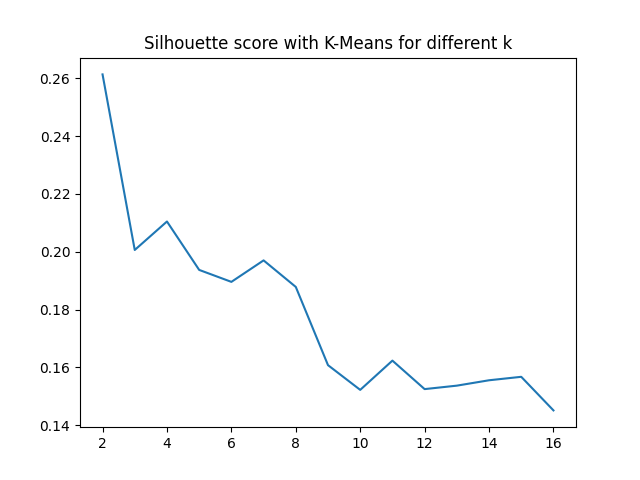
\includegraphics[width=\textwidth]{Imagenes/Bitmap/Clustering/kmeans8sil.png}}%
		\caption{Silhouette Score with K-Means for different $k$}%
		\label{fig:8kmeanssil}
	\end{minipage}
	\hspace{0.4cm}
	\begin{minipage}[b]{0.4\paperwidth}
		\centerline{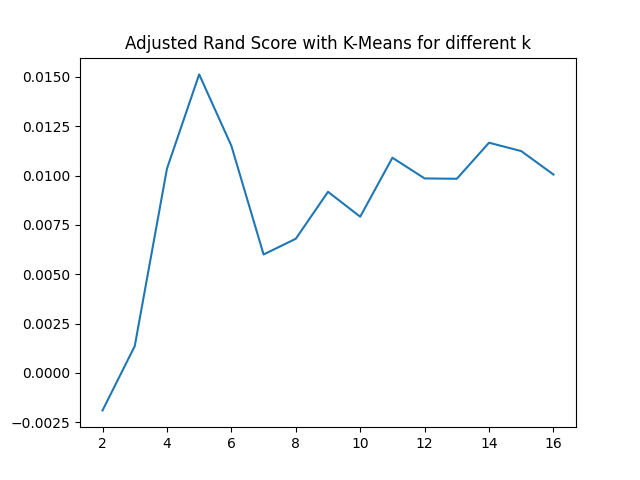
\includegraphics[width=\textwidth]{Imagenes/Bitmap/Clustering/kmeans8ari.png}}%
		\caption{Adjusted Rand Index with K-Means for different $k$}%
		\label{fig:8kmeansari}
	\end{minipage}
\end{figure}

Analysing Figure \ref{fig:8kmeanssil}, which show us the Silhouette Score for different numbers of clusters, we can observe that its result is very similar to the one represented by Figure \ref{fig:nkmeanssil}. As in that case, the best Silhouette Score is obtained when the parameter has the value two. However, this result is far from our classification which has twelve different categories (these were defined Section \ref{sect:DatPrep}). This Silhouette Score means that more than two clusters do not differentiate well enough.

To check how the resulting classification fits with our categorisation, we use the Adjusted Rand Index (as it is described in Figure \ref{fig:8kmeansari}). However, the best result that we are able to obtain is with five cluster and its Adjusted Rand Index is around 0.015. As we know, it is a value very close to zero, what means that there are not enough coincidences in the resulting classification and our categorisation. The rest of the values with other numbers of cluster are worst than this.

After this unfortunate results, we are going to carry out the analysis with DBSCAN algorithm. As we have explained, DBSCAN requires a threshold distance and a minimum number of elements that can create a cluster as parameters. As in Section \ref{sect:clust1}, we are going to assign the value of three to this last parameter and to execute with different $\varepsilon$ values (the threshold distance) for the analysis. Furthermore, as it is possible to execute it with different metrics we are going to try with both euclidean and manhattan distance. Then, the Silhouette Score and Adjusted Rand Index of each execution are calculated.

\begin{figure}
	\centering%
	\centerline{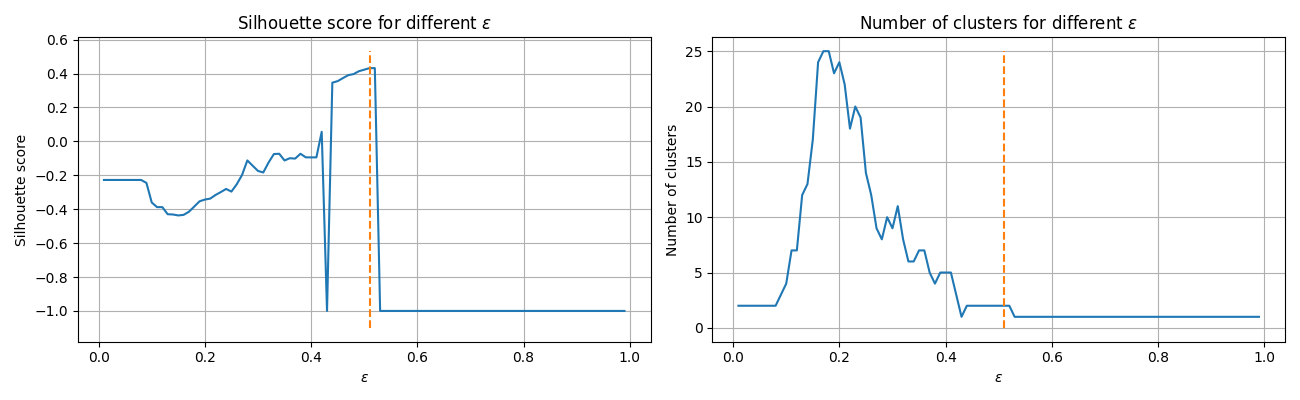
\includegraphics[width=\textwidth]{Imagenes/Bitmap/Clustering/dbscan8sil.png}}%
	\caption{Results of DBSCAN execution with manhattan metric}%
	\label{fig:dbscanman}
\end{figure}

The results of the Silhouette Score calculation with both metrics is very similar. For this reason, we will only show the one with the manhattan distance (see Figure \ref{fig:dbscanman}). In the graph which represent the different Silhouette Score values depending on the taken $\varepsilon$, we are able to see that the maximum value is obtained with a threshold distance that creates two different clusters. As with the K-Means algorithm, this indicates that the best differentiating classification is very far from our categorisation. Once we have observed the same result with these two algorithms, we can claim that our different categories are not different enough for the clustering algorithms with the eight selected dimensions.

\begin{figure}[h]
	\centering%
	\centerline{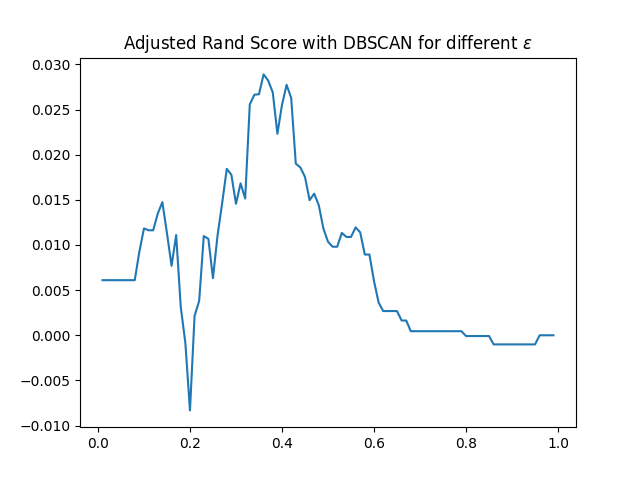
\includegraphics[width=0.5\textwidth]{Imagenes/Bitmap/Clustering/dbscan8ari.png}}%
	\caption{Adjusted Rand Index of DBSCAN with manhattan metric}%
	\label{fig:dbscan8ari}
\end{figure}

As expected, the results of the Adjusted Rand Index are very close to zero again. It can be observed in Figure \ref{fig:dbscan8ari}. The higher Adjusted Rand Index does not achieve the value of 0.03 and the rest of the values are smaller than it. This means that our categorisation does not fit with the returned classification.

In conclusion, the two clustering techniques that we have used for analysing the data with the selected eight dimension do not return a classification similar to that defined by us. However, the results with all features were not initially promising. It could mean that the implemented style markers are not good enough in order to describe the style based on the recipient. Nevertheless, it would be necessary a research with a bigger amount of messages to say that and, perhaps, with a more balanced distribution of each category.